\documentclass[11pt,oneside]{article}
\usepackage[utf8]{inputenc}
\usepackage[a4paper,top=2cm,left=2cm,right=2cm,bottom=2cm]{geometry}
\usepackage{import}
\usepackage[T1]{fontenc}
\usepackage[german,ngerman]{babel}
\usepackage[table]{xcolor}
\usepackage{amsthm, esvect}
\usepackage{mathtools}
\RequirePackage{amssymb, amsfonts, amsmath, latexsym, verbatim, xspace}
\usepackage{systeme}
\usepackage{multicol}
\usepackage{multirow}
\usepackage{framed}
\usepackage{array}
\usepackage{ragged2e}
\usepackage{graphicx}
\usepackage{pdflscape}
\usepackage{epstopdf}
\usepackage{booktabs}
\usepackage{pdfpages}
\usepackage{float} % Allows putting an [H] in \begin{figure} to specify the exact location of the figure
\usepackage{wrapfig} % Allows in-line images such as the example fish picture
\usepackage{tikz, graphicx} % tikz
\usepackage[position=top]{subfig}
\usepackage[bookmarks=true]{hyperref}%Links
\usepackage{enumerate}
\usepackage{enumitem}
\usepackage[german,ruled,vlined,linesnumbered,algosection]{algorithm2e}
\usepackage[labelfont=sf]{caption}
\usepackage{lmodern}
\usepackage{lscape}
\usepackage{tabularx}
\usepackage{systeme}
\usepackage{hhline}
\usepackage{subfiles}
\usepackage{stackengine}
\usepackage{setspace}
\usepackage{MnSymbol}
\usepackage{tcolorbox}
\usepackage{bbm}
\usepackage{url}
\usepackage{xparse}
\usepackage{sectsty}
\usepackage{array}
\usepackage{ragged2e}
\usepackage{listings} %Stellt Code-Snippets sauber dar

% definiert die Sprache
\selectlanguage{German}

% add command for different dates in Swiss fashion
\newcommand{\monthwordlong}[1]{\ifcase#1 \or Januar\or Februar\or März\or April\or Mai\or Juni\or Juli\or August\or September\or Oktober\or November\or Dezember\fi}
\newcommand{\monthwordshort}[1]{\ifcase#1\or Jan\or Feb\or Mar\or Apr\or Mai\or Jun\or Jul\or Aug\or Sept\or Okt\or Nov\or Dez\fi}
\newcommand{\datelong}{\number\day.\:\monthwordlong{\the\month}\:\number\year}
\newcommand{\dateshort}{\number\day.\:\monthwordshort{\the\month}\:\number\year}

% define color of links inside a text
\definecolor{linkblue}{RGB}{0, 0, 80}
\definecolor{plotblue}{RGB}{100, 100, 255}
\definecolor{myblue}{RGB}{8,164,214}
\definecolor{myred}{RGB}{143,42,41}
\definecolor{forestgreen}{RGB}{34,139,34}
\definecolor{highdive}{RGB}{10,169,194}
\definecolor{charcoal}{RGB}{74,74,74}
\hypersetup{
	colorlinks=true,
	linkcolor=linkblue,
	filecolor=magenta,
	urlcolor=plotblue,
	citecolor=linkblue,
	pdfpagemode=FullScreen,
}


\lstdefinestyle{mystyle}{ % definiert den style des Code-Snippets
	%backgroundcolor=\color{backcolour},
	%commentstyle=\color{codegreen},
	%keywordstyle=\color{magenta},
	%numberstyle=\tiny\color{codegray},
	%stringstyle=\color{codepurple},
	basicstyle=\ttfamily\footnotesize,
	breakatwhitespace=false,
	breaklines=true,
	captionpos=b,
	keepspaces=true,
	%numbers=left,
	%numbersep=5pt,
	showspaces=false,
	showstringspaces=false,
	showtabs=false,
	tabsize=4
}
\lstset{style=mystyle}
\usepackage{fancyhdr}

\tcbuselibrary{breakable,skins}
\usetikzlibrary{mindmap,trees}
\newlength\tindent
\setlength{\tindent}{\parindent}
\setlength{\parindent}{0pt}
\renewcommand{\indent}{\hspace*{\tindent}}

\makeatletter
\def\ifEmpty#1{\def\@temp{#1}\ifx\@temp\@empty}
\makeatother

\sectionfont{\underline}
\usetikzlibrary{arrows, petri, topaths, graphs}


% =================== BEISPIEL ====================
\theoremstyle{definition}
\newtheorem{beispiel}{Beispiel}
\renewcommand{\thebeispiel}{\arabic{beispiel}}

% =================== AUFGABE =====================
\newcounter{aufg}[section] % Zähler für die Umgebungen

\newenvironment{aufgabe}[1][]{%
    \refstepcounter{aufg}% Inkrementiere den Zähler
    \begin{tcolorbox}[%
        enhanced,
        overlay unbroken and first={\mytitleaufg[#1]}, % Titelleiste mit Icons wird nicht über Seite gebrochen
        colframe=black,
        boxrule=0pt,
        breakable,
        top=15pt,
        before=\vskip18pt,
    ]
}{%
    \end{tcolorbox}
}

\newcommand{\mytitleaufg}[1][]{% Definiert die Titelleiste und Icons
    \node[fill=black!20,
        rounded corners,
        draw=black,
        text=black,
        line width=1pt,
        inner sep=4pt,
        anchor=west,
        xshift=12pt]
        at (frame.north west){\bfseries Aufgabe \thesection.\theaufg.\ifEmpty{#1}\else\emph{ (#1)}\fi}; % Titel, letzter Teil mit ifempty testet ob #1 leer und macht Klammern und Titel, falls Titelargument übergeben wird bzw. falls #1 leer erscheint nichts - auch keine Klammern

    \node[% Icon
        rounded corners,
        text=black,
        fill=black,
        line width=0pt,
        inner sep=3pt,
        anchor=west,
        xshift=5pt,
        % yshift=-35pt
        ]
        at (frame.north east){
\includegraphics[width=24pt]{../../../Header/Icons/aufgabeicon.png}};
}

% =================== DEFINITION ==================
\newcounter{def}[section] % Zähler für die Umgebungen

\newenvironment{definition}[1][]{%
    \refstepcounter{def}% Inkrementiere den Zähler
    \begin{tcolorbox}[%
        enhanced,
        drop shadow southeast,
        overlay unbroken and first={\mytitledef[#1]}, % Titelleiste mit Icons wird nicht über Seite gebrochen
        colback=blue!5!white,
        colframe=blue!75!black,
        boxrule=2pt,
        breakable,
        top=15pt,
        before=\vskip18pt,
    ]
}{%
    \end{tcolorbox}
}

\newcommand{\mytitledef}[1][]{% Definiert die Titelleiste und Icons
    \node[fill=blue!40!white,
        rounded corners,
        draw=black,
        text=black,
        line width=1pt,
        inner sep=4pt,
        anchor=west,
        xshift=12pt]
        at (frame.north west){\bfseries Definition \thesection.\thedef.\ifEmpty{#1}\else\emph{ (#1)}\fi}; % Titel, letzter Teil mit ifempty testet ob #1 leer und macht Klammern und Titel, falls Titelargument übergeben wird bzw. falls #1 leer erscheint nichts - auch keine Klammern

    \node[% Icon
        rounded corners,
        text=black,
        fill=black,
        line width=0pt,
        inner sep=3pt,
        anchor=west,
        xshift=5pt,
        % yshift=-35pt
        ]
        at (frame.north east){
\includegraphics[width=24pt]{../../../Header/Icons/definitionicon.png}};
}

% =================== NOTATION ====================
\newcounter{nota}[section] % Zähler für die Umgebungen

\newenvironment{notation}[1][]{%
    \refstepcounter{nota}% Inkrementiere den Zähler
    \begin{tcolorbox}[%
        enhanced,
        drop shadow southeast,
        colback=yellow!5!white,
        colframe=yellow!75!black,
        overlay unbroken and first={\mytitlenota[#1]},   % Titelleiste mit Icons wird nicht über Seite gebrochen
        boxrule=2pt,
        breakable,
        top=15pt,
        before=\vskip18pt,
    ]
}{%
    \end{tcolorbox}
}

\newcommand{\mytitlenota}[1][]{% Definiert die Titelleiste und Icons
    \node[fill=yellow!40!white,,
        rounded corners,
        draw=black,
        text=black,
        line width=1pt,
        inner sep=4pt,
        anchor=west,
        xshift=12pt]
        at (frame.north west){\bfseries Notation \thesection.\thenota.\ifEmpty{#1}\else\emph{ (#1)}\fi}; % Titel, letzter Teil mit ifempty testet ob #1 leer und macht Klammern und Titel, falls Titelargument übergeben wird bzw. falls #1 leer erscheint nichts - auch keine Klammern

    \node[% Icon
        rounded corners,
        text=black,
        fill=black,
        line width=0pt,
        inner sep=3pt,
        anchor=west,
        xshift=5pt,
        % yshift=-35pt
        ]
        at (frame.north east){
\includegraphics[width=24pt]{../../../Header/Icons/definitionicon.png}};
}

% =================== SATZ ========================
\newcounter{satz}[section]  % creates a counter and resets it after each chapter

\newenvironment{satz}[1][]{   % Hauptbox mit Satz drin
    \refstepcounter{satz}
    \begin{tcolorbox}[%
        enhanced,
        colback=red!5!white,
        fuzzy halo=2mm with gray,
        colframe=red!75!black,
        overlay unbroken and first={\mytitlesatz[#1]},   % Titelleiste mit Icons wird nicht über Seite gebrochen
        boxrule=2pt,
        breakable,
        top=15pt,
        before=\vskip18pt,
    ]
}{%
    \end{tcolorbox}
}

\newcommand{\mytitlesatz}[1][]{                     % Macht Titelbox und Icons
   \node[fill=red!90!white,
      rounded corners,
      draw=black,,
      text=black,
      line width=1pt,
      inner sep=4pt,
      anchor=west,
      xshift=12pt]
   at (frame.north west){\bfseries Satz \thesection.\thesatz.\ifEmpty{#1}\else\emph{ (#1)}\fi};  % Titel, letzter Teil mit ifx testet ob #1 leer und macht Klammern und Titel, falls Titelargument übergeben wird bzw.  falls #1 leer erscheint nichts - auch keine Klammern

 \node[ % Icon
      rounded corners,
      text=black,
      fill=black,
      line width=0pt,
      inner sep=3pt,
      anchor=west,
      xshift=5pt,
%     yshift=-35pt
]
   at (frame.north east){ 
\includegraphics[width=24pt]{../../../Header/Icons/satzicon.png} };
}

% =================== BEWEIS ======================
\newenvironment{beweis}[1][]{
    \begin{tcolorbox}[
        enhanced,
        overlay unbroken and first={\mybeweis[#1]},     % Titelleiste mit Icons wird nicht über Seite gebrochen
        colback=white,
        colframe=black,
        boxrule=0pt,
        breakable,
        top=15pt,
        before=\vskip18pt,
    ]
}{
        \end{tcolorbox}
}

\newcommand{\mybeweis}[1][]{                     % Macht Titelbox und Icons
   \node[fill=white,
      rounded corners,
      draw=black,
      text=black,
      line width=1pt,
      inner sep=4pt,
      anchor=west,
      xshift=12pt]
   at (frame.north west){\bfseries Beweis \ifEmpty{#1}\else\emph{ (#1)}\fi};  % Titel, letzter Teil mit ifx testet ob #1 leer und macht Klammern und Titel, falls Titelargument übergeben wird bzw.  falls #1 leer erscheint nichts - auch keine Klammern
}

% =================== ALGORITHM ===================
\newcounter{algo}[section]  % creates a counter and resets it after each chapter

\newenvironment{algo}[1][]{   % Hauptbox mit Satz drin
    \refstepcounter{algo}
    \begin{tcolorbox}[%
        enhanced,
        drop shadow southeast,
        colback=yellow!5!white,
        colframe=yellow!75!black,
        overlay unbroken and first={\algotitle[#1]},   % Titelleiste mit Icons wird nicht über Seite gebrochen
        boxrule=2pt,
        breakable,
        top=15pt,
        before=\vskip18pt,
    ]
}{%
    \end{tcolorbox}
}

\newcommand{\algotitle}[1][]{                     % Macht Titelbox und Icons
   \node[fill=yellow!40!white,
      rounded corners,
      draw=black,
      text=black,
      line width=1pt,
      inner sep=4pt,
      anchor=west,
      xshift=12pt]
   at (frame.north west){\bfseries \ifEmpty{#1}{Ablauf}\else{#1}\fi};  % Titel, letzter Teil mit ifx testet ob #1 leer und macht Klammern und Titel, falls Titelargument übergeben wird bzw.  falls #1 leer erscheint nichts - auch keine Klammern

 \node[ % Icon
      rounded corners,
      text=black,
      fill=black,
      line width=0pt,
      inner sep=3pt,
      anchor=west,
      xshift=5pt
      % yshift=-35pt
      ]
   at (frame.north east){ 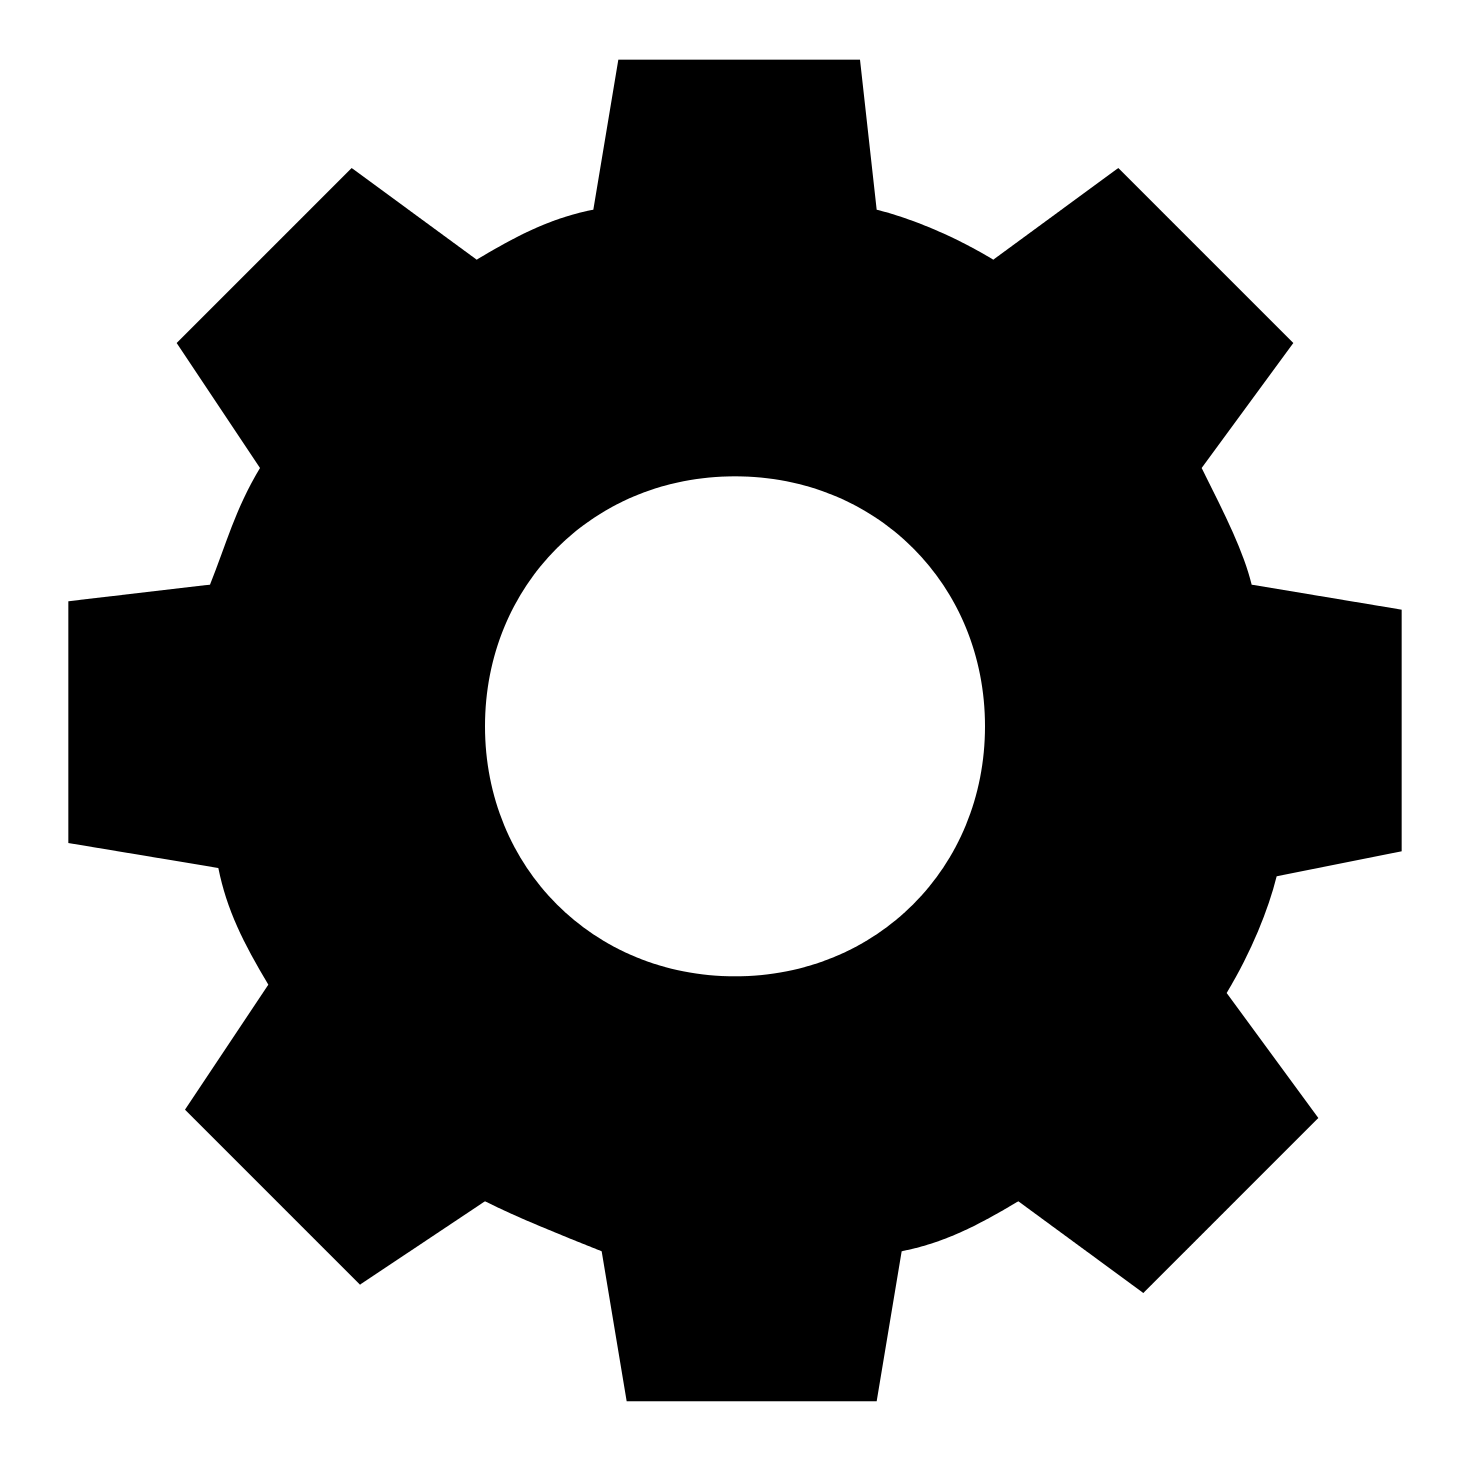
\includegraphics[width=24pt]{../../../Header/Icons/algoicon.png} };
}

% ================ Nummerierte Multicol ================
\newenvironment{enumcols}[1][]{
    \begin{enumerate}[label=\alph*)]\begin{multicols}{#1}
}{
    \end{multicols}\end{enumerate}
}



% =================================================
\usetikzlibrary{shapes,arrows}
\tikzstyle{decision} = [diamond, draw, fill=blue!20,
    text width=6em, text badly centered, node distance=4cm, inner sep=0pt]
\tikzstyle{block} = [rectangle, draw, fill=blue!20,
    text width=8em, text centered, rounded corners, minimum height=4em]
\tikzstyle{line} = [draw, -latex']
\tikzstyle{cloud} = [draw, ellipse,fill=red!20, node distance=2cm,
    minimum height=2em]

% Karriertes Papier für Antwort
\newcommand{\karos}[1]{\begin{tikzpicture}\draw[step=0.5cm,color=gray] (0,0) grid (\linewidth,#1 cm);\end{tikzpicture}}
%%
% Header and Footer
%%
\linespread{1.2} % Line spacing
\fancypagestyle{plain}{
	\pagestyle{fancy}
	\lhead{}
	\chead{}
	\rhead{}
	\lfoot{\Autor}
	\cfoot{\Skriptname}
	\rfoot{\thepage}
	\renewcommand{\headrulewidth}{0pt}
	\renewcommand{\footrulewidth}{0.4pt}
}

\pagestyle{fancy}
\fancyhf{}
\rhead{\rightmark}
\lfoot{\leftmark}
\rfoot{\thepage}
\renewcommand{\headrulewidth}{0.2pt}
%\setlength\parindent{0pt} % Uncomment to remove all indentation from paragraphs



%%
% Math Arrows
%%
\newcommand{\same}{\ensuremath{\Longleftrightarrow}}
\renewcommand{\to}{\ensuremath{\longrightarrow}}
\newcommand{\qsame}{\quad\same\quad}
\newcommand{\dsame}{\ensuremath{:\Leftrightarrow}}
\newcommand{\qdsame}{\quad\dsame\quad}
\newcommand{\ldsame}{\ensuremath{:\Longleftrightarrow}}
\newcommand{\samedef}{\ensuremath{\us {\text{def}} \Leftrightarrow}}
\newcommand{\qsamedef}{\quad\samedef\quad}
\newcommand{\lsamedef}{\ensuremath{\us {\text{def}} \Longleftrightarrow}}
\newcommand{\qlsamedef}{\quad\lsamedef\quad}


%%
% Mengendefinitionen
%%
\newcommand{\M}{\ensuremath{\mathcal{M}}}
\newcommand{\N}{\ensuremath{\mathbb{N}}}
\newcommand{\Z}{\ensuremath{\mathbb{Z}}}
\newcommand{\Q}{\ensuremath{\mathbb{Q}}}
\newcommand{\I}{\ensuremath{\mathbb{I}}}
\newcommand{\R}{\ensuremath{\mathbb{R}}}
\newcommand{\C}{\ensuremath{\mathbb{C}}}
\renewcommand{\S}{\ensuremath{\mathbb{S}}}
\newcommand{\Prim}{\ensuremath{\mathbb{P}}}
\newcommand{\0}{\ensuremath{\emptyset}}
\renewcommand{\Re}{\ensuremath{\operatorname{Re}}}
\renewcommand{\Im}{\ensuremath{\operatorname{Im}}}
\newcommand{\strich}{\ensuremath{\big\vert}}

%%
% Mengenoperation
%%
\renewcommand{\nin}{\not\in}


%%
% Logisches Und und Oder
%%
\newcommand{\sand}{\ensuremath{\; \land \;}}
\newcommand{\sor}{\ensuremath{\; \lor \;}}
\renewcommand{\*}{\ensuremath{\cdot}}
\newcommand{\oder}{\vee}
\newcommand{\n}{\neg}
\newcommand{\und}{\wedge}


%%
% Bei Integral, Summe,... die Grenzen über bzw.
% unter das Zeichen
%%
\renewcommand{\d}[1]{\ensuremath{\operatorname{d}\!{#1}}}
\newcommand{\Sum}{\sum\limits}
\newcommand{\Prod}{\prod\limits}
\newcommand{\Min}{\min\limits}
\newcommand{\Max}{\max\limits}
\newcommand{\Lim}{\lim\limits}
\newcommand{\Inf}{\inf\limits}
\newcommand{\Sup}{\sup\limits}
\newcommand{\Liminf}{\liminf\limits}
\newcommand{\Limsup}{\limsup\limits}
%\renewcommand{\Cup}{\bigcup\limits}
%\renewcommand{\Cap}{\bigcap\limits}
\newcommand{\Otimes}{\bigotimes\limits}
\newcommand{\Oplus}{\bigoplus\limits}


%%
% Arcus Cotangens, Logarithmus
%%
\let\oldsin\sin
\renewcommand{\sin}[1]{\oldsin{\left(#1\right)}}
\let\oldcos\cos
\renewcommand{\cos}[1]{\oldcos{\left(#1\right)}}
\let\oldtan\tan
\renewcommand{\tan}[1]{\oldtan{\left(#1\right)}}
\let\oldarcsin\arcsin
\renewcommand{\arcsin}[1]{\oldarcsin{\left(#1\right)}}
\let\oldarccos\arccos
\renewcommand{\arccos}[1]{\oldarccos{\left(#1\right)}}
\let\oldarctan\arctan
\renewcommand{\arctan}[1]{\oldarctan{\left(#1\right)}}
\let\oldln\ln
\renewcommand{\ln}[1]{\oldln{\left(#1\right)}}
\newcommand{\Log}[2]{\ensuremath{\operatorname{log}_{#1}\left(#2\right)}}
\newcommand{\e}{\operatorname{e}}
\renewcommand{\exp}[1]{\ensuremath{\operatorname{\e}^{#1}}}


%%
% Griechische Buchstaben
%%
\renewcommand{\epsilon}{\ensuremath{\varepsilon}}
\renewcommand{\phi}{\varphi}
\renewcommand{\l}{\lambda}
\renewcommand{\t}{\tau}


%%
% Bezeichnungen
%%
\newcommand{\Rgn}{\R_{>0}} % R grösser Null
\newcommand{\Rad}{\operatorname{Rad}}   % Radikal
\newcommand{\kgV}{\operatorname{kgV}}   % Kleinster gemeinsame Vielfache
\newcommand{\ggT}{\operatorname{ggT}}   % Grösster gemeinsame Teiler
\newcommand{\winkel}{\sphericalangle}          % Winkelsymbol
\DeclarePairedDelimiter\abs{\lvert}{\rvert} % besserer Betrag
\makeatletter
\let\oldabs\abs
\def\abs{\@ifstar{\oldabs}{\oldabs*}}
\makeatother


%%
% Vektorgeometrie
%%
\renewcommand{\v}[1]{\vv{#1}}       % besserer Pfeil über Buchstaben
\renewcommand{\vec}[2]{\begingroup\renewcommand{\arraystretch}{1}\left(\begin{array}{c} #1 \\ #2 \end{array}\right)\endgroup}   % two dimensional vector
\renewcommand{\Vec}[3]{\begingroup\renewcommand{\arraystretch}{1}\left(\begin{array}{c} #1 \\ #2 \\ #3 \end{array}\right)\endgroup}      % three dimensional vector


%%
% Text
%%
\newcommand*{\Ueq}[1]{\mathrel{\mathop{=}\limits_{\text{#1}}}}
\newcommand*{\Oeq}[1]{\mathrel{\stackrel{\text{#1}}{=}}}
\newcommand{\utext}[2]{\underbrace{#1}_{\substack{#2}}}
\newcommand{\otext}[2]{$\overbrace{\textrm{#1}}^{\textrm{#2}}$}
\newcommand{\lineortext}[1]{\hspace{0,1cm}\underline{\hspace{0.1cm}\hphantom{#1}\hspace{0.1cm}}\hspace{0,1cm}} % Lückentext erstellen
\newcommand{\gap}[1]{\rule{#1 cm}{1pt}}


\newcommand{\Skriptname}{Die Grundlagen des Kreises}
\newcommand{\Autor}{Jonas Guler (Gu)}
\newcommand{\version}{\textit{v}1.0}
\graphicspath{{images/}} % set path to image directory

\begin{document}
\begin{titlepage}
	\clearpage
	\title{\Huge\textbf{\Skriptname} \\[1cm]}
	\author{Autor:\\ \Autor}
	\date{\normalsize {Version \version}\\ \datelong}
	\maketitle
	\thispagestyle{empty}
	\vfill
	\tableofcontents
\end{titlepage}
\pagenumbering{arabic}
%############################################################################################
\section{Der Kreis}
\subsection{Kreisumfang}
	Wie bestimmt man bei gegebenem Durchmesser den Umfang eines Kreises?\newline
	Dies ist wohl die älteste Frage der Geometrie. Deshalb wollen wir ihr natürlich auf den Grund gehen.
	\begin{aufgabe}
		Berechne in den folgenden Teilaufgaben jeweils den Bruch $\frac{\text{Umfang}}{\text{Durchmesser}}$. Was fällt dir dabei auf?
		\begin{enumcols}[3]
			\item $d=2,\quad U=6.283$
			\item $d=3.4,\quad U=10.681$
			\item $d=0.3,\quad U=0.942$
		\end{enumcols}
		Wir stellen also fest, dass folgender Zusammenhang gilt:
		\[\lineortext{\frac{\text{Umfang}}{\text{Durchmesser}}=\text{konstant}}.\]
	\end{aufgabe}
	Wir sehen also die Grösse des Kreises spielt in der obigen Gleichung keine Rolle. In jedem Fall erhalten wir die gleiche konstante Zahl.
	Betrachten wir die Formel für den Umfang eines Kreises, so stellen wir fest, um welche bekannte Zahl es sich handelt.
	\begin{satz}[Kreisumfang]
		Der Umfang eines Kreises mit Radius $r$ beträgt \[U=\lineortext{d\cdot\pi=2r\cdot\pi}.\]
	\end{satz}
	Wagen wir gemeinsam einen Blick in die Vergangenheit und versuchen zu verstehen, wie diese konstante Zahl $\pi$ näherungsweise gefunden wurde. Bereits verschiedene Völker der Antike haben verschiedene Näherungswerte gefunden.
	\begin{aufgabe}
		\begin{minipage}{0.6\linewidth}\begin{enumerate}[label=\ ]
				\item Ägypter ($1900$ v. Chr.)
				\item Babylonier ($2$. Jahrtausend v. Chr.)
				\item Inder ($500$ v. Chr.)
				\item Platon ($427-348$ v. Chr.)
				\item Zhang Heng \& Brahmagupta ($7$. Jhd)
		\end{enumerate}\end{minipage}\hfill\begin{minipage}{0.4\linewidth}\begin{enumerate}[label=\ ]
				\item $\left(\frac{4}{3}\right)^4=$
				\item $\frac{25}{8}=$
				\item $\left(\frac{26}{15}\right)^2=$
				\item $\sqrt{2}+\sqrt{3}=$
				\item $\sqrt{10}=$
		\end{enumerate}\end{minipage}
	\end{aufgabe}
	\begin{figure}[H]
		\centering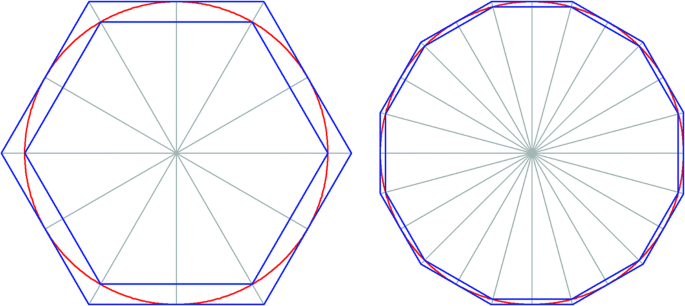
\includegraphics[scale=0.25]{6-12EckArchimedes.png}
		\caption{Archimedes' einbeschriebene 6-Eck links und rechts mit einem 12-Eck}
		\label{fig:Archi6-12e}
	\end{figure}
	Die erste systematische Berechnung von $\pi$ absolvierte Archimedes ($287-212$ v. Chr.), in dem er den Kreis zwischen regelmässigen Vielecken einzwängt. Dabei startete er mit zwei $6$-Ecken, welche einem Kreis mit Durchmesser $1$ eingeschrieben werden, bzw. umschliessen (siehe Abbildung \ref{fig:Archi6-12e}) und verdoppelte danach die Anzahl Ecken viermal bis zum $96$-Eck. Nun berechnetet er für jedes Vieleck jeweils den Umfang des äusseren und des inneren und konnte so die Zahl $\pi$ annähern.\newline
	Die Formel für den Interationsschritt (von $n$ nach $2n$-Ecken) lautet:
	\begin{equation}\label{eq:iterArchi}
		U_{2n}=\frac{2\cdot U_n}{\sqrt{2+2\sqrt{1-\left(\frac{U_n}{n}\right)^2}}},
	\end{equation}
	wobei $n$ die Anzahl Ecken, $U_n$ der Umfang des regelmässigen $n$-Ecks und $U_{2n}$ der Umfang des regelmässigen $2n$-Ecks entspricht.
	\begin{aufgabe}
		Versuche nun den Iterationsweg von Archimedes mit Hilfe deines Taschenrechners nachzuvollziehen. Es soll der Umfang eines Kreises mit Durchmesser $d=1$ angenähert werden. Dabei wissen wir, dass der Umkreisradius eines Sechsecks gleich lang ist, wie die Seitenlänge. Das bedeutet, wir starten mit dem inneren $6$-Eck mit Seitenlänge $s=0.5$, also einem Umfang von $U_6=3$. Benutze die Formel \ref{eq:iterArchi}, um die Tabelle unten zu vervollständigen.
		\begingroup\renewcommand{\arraystretch}{1.5}
		\begin{table}[H]
			\centering
			\begin{tabular}{c|p{6cm}}
				Eckenzahl $n$ & Umfang $U_n$ \\\hline
				$6$ & $3$ \\\hline
				$12$ & \\\hline
				$24$ & \\\hline
				$48$ & \\\hline
				$96$ & \\\hline
				$192$ & \\\hline
				$384$ & \\
			\end{tabular}
		\end{table}
		\endgroup
	\end{aufgabe}
	Der Kreis mit Durchmesser $d=1$ hat also einen Umfang von $U=\pi=3.14159265\ldots$. Halten wir also fest:
	\begin{definition}
		Die Kreiszahl $\pi$ entspricht für jeden Kreis dem Quotient $\frac{\text{Umfang}}{\text{Durchmesser}}$ und beträgt konstant \[\pi=3.14159265\ldots\]
	\end{definition}
	Leider wird diese Methode zur Berechnung von $\pi$ heute nicht mehr verwendet, da die Berechnung mit unendlichen Summen oder unendlichen Produkten viel effizienter und vorallem für den Computer einfacher ist. Jedoch kann man damit $\pi$ beliebig genau berechnen.


\subsection*{Fun Facts: (Stand $2023$)}
	\begin{itemize}
		\item \url{https://www.angio.net/pi}, \url{https://www.piday.org/million}
		\item Bis heute hat die Fachhochschule Graubünden den Weltrekord für die meisten berechneten Nachkommastellen von $\pi$ inne. Sie haben $62.8$ Billionen Stellen nach dem Komma berechnet.\newline Den Weltrekord für die meisten auswendig aufgesagten Nachkommastellen hält der Inder Suresh Kumar Sharma mit $70'030$ Stellen nach dem Komma.
		\item Betrachten wir ein Quadrat mit Seitenlänge $s=1$ und in diesem Quadrat einen Viertelkreis mit Radius $r=1$. Die \textcolor{red}{Länge des Viertelkreises} ist $\frac{2r\pi}{4}=\frac{\pi}{2}$. Der \textcolor{blue}{halbe Umfang des Quadrats} hat die Länge $1+1=2$. Nun zerstückeln wir diese beiden äusseren Strecken und machen daraus eine Treppe. Die Länge der beiden horizontalen Linien zusammen beträgt immer noch 1, ebenso die Länge der beiden vertikalen Linien zusammen. Diese Treppenlinie hat also insgesamt immer noch die Länge 2. Diese Treppenlinie kann man nun (fast) beliebig formen. Wichtig ist einfach, dass die Striche immer senkrecht zueinander verlaufen. Die Summe aller horizontalen Linien beträgt immer 1, ebenso die Summe der vertikalen Linien. Insgesamt wird die Treppenlinie also immer die Länge 2 haben, egal, wie nahe wir sie an den Viertelkreis \glqq anschmiegen\grqq. Somit bekämen wir im Unendlichen dann: \[1+1=\frac{\pi}{2}\quad\to\quad\pi=4.\]
		\begin{figure}[ht]
			\begin{minipage}{0.3\linewidth}
				\centering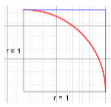
\includegraphics[scale=0.7]{pi4_1.png}
			\end{minipage}
			\hfill
			\begin{minipage}{0.3\linewidth}
				\centering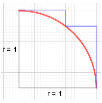
\includegraphics[scale=0.8]{pi4_2.png}
			\end{minipage}
			\hfill
			\begin{minipage}{0.3\linewidth}
				\centering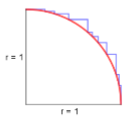
\includegraphics[scale=0.7]{pi4_3.png}
			\end{minipage}
			\caption{Approximation des Kreises mittels senkrechter Linien}
			\label{fig:pi4}
		\end{figure}
	\end{itemize}
	\begin{aufgabe}
		Der Umfang der Erde am Äquator beträgt $40'076$ km. (Die Erde werde hier als Kugel idealisiert.)
		\begin{enumerate}[label=\alph*)]
			\item Berechne den Äquatorradius $r$.\newline\karos{2}
			\item \begin{minipage}{0.6\linewidth}
				Denke dir eine Schnur, die um den Äquator gelegt wird. Diese Schnur ist nun $10$ Meter zu lang. Um sie zu spannen, müsste sie rundherum gleich viel von der Erde angehoben werden. Wie gross muss der Abstand zur Erdoberfläche sein? Schätze zuerst!
			\end{minipage}
			\hfill
			\begin{minipage}{0.35\linewidth}
				\begin{figure}[H]
					\centering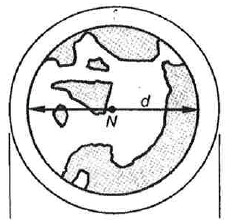
\includegraphics[scale=0.4]{ErdeMitSchnur.png}
				\end{figure}
			\end{minipage}
			\karos{2.5}
		\end{enumerate}
	\end{aufgabe}
	\begin{aufgabe}
		Berechne die Längen dieser Linien.
		\begin{figure}[H]
			\centering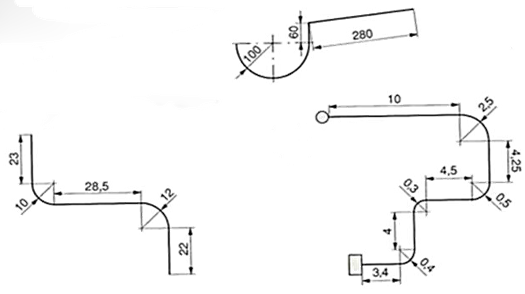
\includegraphics[scale=0.6]{AufgUmfang.png}
		\end{figure}
	\end{aufgabe}

\subsection{Kreisfläche}
	Um die  Fläche eines Kreises zu berechnen, wenn man seinen Radius kennt, kann man folgenden Trick anwenden:
	\begin{aufgabe}
		Betrachte das folgende \href{https://www.geogebra.org/m/gpcvcgxc}{Geogebra-Applet}\footnotemark.
		\begin{enumerate}[label=\alph*)]
			\item Erkläre die Konstruktion des Rechtecks aus dem Kreis.
			\item Begründe, warum der Flächeninhalt des Rechtecks sich bei feinerer Unterteilung (Schieberegler) immer mehr der Größe des Flächeninhalt des Kreises annähert.
			\item Stelle eine Formel für den Flächeninhalt des Rechtecks auf. Benutze dabei die Formel für den Umfang des Kreises mit Radius $r$. \textbf{Tipp:} Seite mal Seite ;-)
		\end{enumerate}
	\end{aufgabe}
	\footnotetext{\url{https://www.geogebra.org/m/gpcvcgxc}}
	\begin{satz}[Kreisfläche]
		Der Flächeninhalt eines Kreis mit Radius $r$ beträgt also: \[\lineortext{A=r^2\pi}.\]
	\end{satz}
	\begin{aufgabe}
		\begin{enumerate}[label=\alph*)]
			\item Welchen Flächeninhalt hat ein Kreis mit Durchmesser $d=10$ cm?
			\item Welchen Durchmesser hat ein Kreis mit Flächeninhalt $A=10$ cm$^2$?
			\item Welchen Flächeninhalt hat ein Kreis mit Umfang $U=20$ cm?
			\item Welchen Umfang hat ein Kreis mit Flächeninhalt $A=20$ cm$^2$?
		\end{enumerate}
	\end{aufgabe}
	\begin{aufgabe}
		Berechne den Inhalt und den Umfang der folgenden grauen Flächen.
		\begin{figure}[H]
			\centering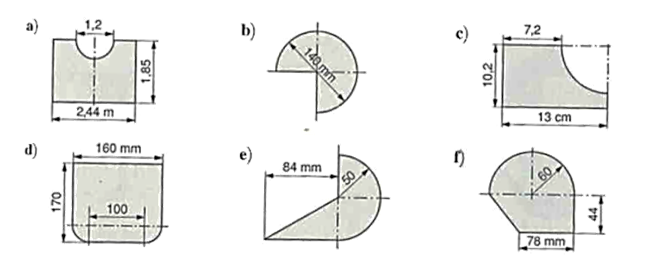
\includegraphics[scale=0.6]{AufgFläche.png}
		\end{figure}
	\end{aufgabe}


\subsection{Kreisbogen und Kreissektor}
	Starten wir mit einer kurzen Aufgabe aus der realen Welt.
	\begin{aufgabe}
		Bearbeite das \href{https://www.geogebra.org/m/pyvvjumu}{Geogebra-Applet}\footnotemark\:und notiere deine Überlegungen.\vspace{5pt}\newline
		\karos{4}
	\end{aufgabe}
	\footnotetext{\url{https://www.geogebra.org/m/pyvvjumu}}
	Die wichtigste Erkenntnis aus der obigen Aufgabe ist:
	\begin{center}\lineortext{Der Mittelpunktswinkel $\alpha$ ist proportional zur Bogenlänge $b$.}\end{center}
	Das heisst: \[\frac{b}{U}=\frac{\alpha}{360^\circ}\quad\to\quad b=\lineortext{\frac{\alpha}{360^\circ}\cdot 2r\pi}.\]
	\begin{satz}[Bogenlänge]
		\begin{minipage}{0.65\linewidth}
			Ein Kreisbogen mit Radius $r$ und Mittelpunktswinkel $\alpha$ hat die Länge \[b=\lineortext{\frac{\alpha}{180^\circ}\cdot r\cdot\pi}.\]
		\end{minipage}
		\hfill
		\begin{minipage}{0.3\linewidth}
			\centering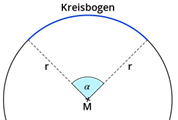
\includegraphics[scale=0.5]{Kreisbogen.png}
		\end{minipage}
		\textit{Beachte: Mit $\alpha=360^\circ$ erhälst du wieder die Formel für den Umfang des Kreises.}
	\end{satz}
	\begin{aufgabe}
		\begin{enumerate}[label=\alph*)]
			\item Die Entfernung der Sonne zur Erde beträgt $150$ Millionen Kilometer. Welchen Weg legt die Erde in einem Tag auf ihrer Kreisbahn um die Sonne zurück?
			\item Ein Satellit umkreist die Erde in $280$ km Höhe über der Erdoberfläche. Für eine komplette Umkreisung braucht er $1.5$ Stunden. Welchen Weg legt der Satellit in einer Stunde zurück? Welche Bahngeschwindigkeit (in km/s) hat der Satellit? \textbf{Tipp: } Erdradius = 6370 km
		\end{enumerate}
		\karos{4}
	\end{aufgabe}
	Mit einer ähnlichen Überlegung können wir die Fläche eines Kreissektors herleiten. Auch hier ist die Fläche proportional zur Winkel. Das heisst:
	\[\frac{A_s}{A}=\frac{\alpha}{360^\circ}\quad\to\quad A_s=\frac{\alpha}{360^\circ}\cdot A=\frac{\alpha}{360^\circ}\cdot r^2\pi\]
	Für die Sektorfläche gibt es aber auch eine zweite Formel, die man bekommt, wenn man die obige Formel mit der Bogenlänge kombiniert:
	\[A_s=\frac{\alpha}{360^\circ}\cdot r\cdot r\cdot\pi=\frac{1}{2}\cdot\utext{\frac{\alpha}{360^\circ}\cdot 2r\cdot\pi}{=b}\cdot r=\frac{1}{2}\cdot b\cdot r\]
	Bemerke das die Formel sehr ähnlich ist zum Dreieck, wobei die Bogenlänge als Grundlinie und der Radius als Höhe interpretiert werden kann.
	\begin{satz}[Sektorfläche]
		\begin{minipage}{0.65\linewidth}
			Ein Kreissektor mit Radius $r$ und Mittelpunktswinkel $\alpha$ hat den Flächeninhalt \[A_s=\frac{\alpha}{360^\circ}\cdot r^2\cdot\pi=\frac{1}{2}\cdot b\cdot r\]
		\end{minipage}
		\hfill
		\begin{minipage}{0.3\linewidth}
			\centering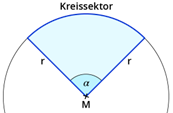
\includegraphics[scale=0.5]{Kreissektor.png}
		\end{minipage}
	\end{satz}
	\begin{aufgabe}
		Berechne den Umfang und den Flächeninhalt folgender Figuren. Gib das Resultat in Abhängigkeit der Gitterlänge an.
		\begin{figure}[H]
			\centering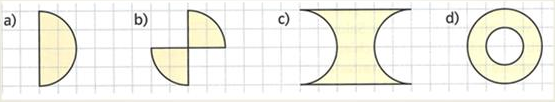
\includegraphics[scale=0.7]{AufgSekBog.png}
		\end{figure}
		\karos{4}
	\end{aufgabe}
	\newpage


\section{Das Bogenmass}
	In diesem Abschnitt möchte wir neben Grad ein neues Winkelmass einführen. Dieses hat grosse Vorteile und wird deshalb vorallem in der höheren Mathematik, naturwissenschaftlichen und technischen Anwendungen im internationalen Froschungsbereich verwendet. Eine Idee für dieses neue Winkelmass wäre, einfach die Bogenlänge des zum Winkel gehörenden Kreissektors als Einheit zu verwenden. Dabei ergibt sicher aber noch eine kleine Herausforderung. Die Bogenlänge ist abhängig von Radius des Kreissektors. Um dies zu umgehen, haben sich die Mathematiker wieder an ihrem Lieblingstrick bedient. Sie wählen den Radius $r=1$, damit er in der Berechung ignoriert werden kann.
	\begin{definition}
		\begin{minipage}{0.55\linewidth}
			Betrachte einen Kreis mit Radius $r=1$ um den Ursprung. Die \textcolor{green}{Bogenlänge} des zum Winkel gehörenden Kreissektors definiert das Bogenmass. \newline
			Das heisst: der Winkel $45^\circ$ entspricht \lineortext{$\quad0.79\quad$} im Bogenmass.
		\end{minipage}
		\hfill
		\begin{minipage}{0.4\linewidth}
			\begin{figure}[H]
				\centering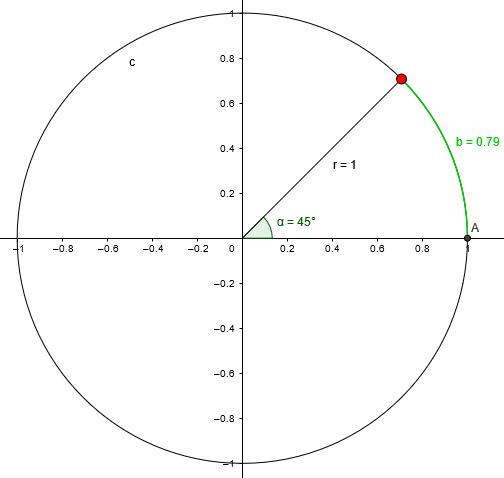
\includegraphics[scale=0.29]{Einheitskreis.png}
			\end{figure}
		\end{minipage}
	\end{definition}
	\begin{aufgabe}
		\begin{enumerate}
			\item Ein $360^\circ$ Winkel entspricht, wie viel im Bogenmass? Erkläre deine Lösung.
			\item Fülle die folgende Tabelle aus.
			\begin{table}[H]
				\centering
				\begin{tabular}{m{3cm}|m{0.6cm}|m{0.6cm}|m{0.6cm}|m{0.6cm}|m{0.6cm}|m{0.6cm}|m{0.6cm}|c|m{0.6cm}}
					Winkel in Grad & $0$ & $360$ & $\:\:1$ & $\:90$ & $180$ & $270$ & $\:33$ & & \\\hline
					Winkel in Bogenmass & $0$ & & & & & & & $1.5708$ & $1$ \\\hline
					Winkel als Vielfaches von $\pi$ & $0$ & & $\:\:$X & $\:\frac{\pi}{2}$ & & & $\:\:$X & X & $\:\:$X \\
				\end{tabular}
			\end{table}
			\item Überprüfe deine Berechnungen aus der Tabelle, indem du im \href{https://www.geogebra.org/m/wwh8jhtm}{Geogebra-Applet}\footnotemark\:den roten Punkt auf dem Kreis verschiebst.
		\end{enumerate}
		\karos{4}
	\end{aufgabe}
	\footnotetext{\url{https://www.geogebra.org/m/wwh8jhtm}}
	\subsection*{Wie können wir nun aber Grad in Bogenmass umrechnen?}
	Wir betrachten dafür die Formel für die Bogenlänge:
	\begin{equation*}
		\begin{aligned}[c]
			\textcolor{green}{b}=\frac{\alpha}{360^\circ}\cdot2\pi\cdot r
		\end{aligned}
		\qquad\to\qquad
		\begin{aligned}[c]
			\alpha=\frac{360^\circ\cdot\textcolor{green}{b}}{2\pi \cdot r}=\frac{180^\circ}{\pi}\approx 57.3^\circ
		\end{aligned}
	\end{equation*}
	Bemerke, dass in der Berechnung oben die Länge des Radius und des Bogens keine Rolle spielen, Solange sie gleich gross sind. Das heisst, für den speziellen Winkel $\alpha=57.3^\circ$ ist die Bogenlänge gleich wie der Radius. Deshalb wird dieser Winkel auch mit $1$ rad bezeichnet.
	\begin{satz}
		\begin{minipage}{0.55\linewidth}
			Für die Umrechnung von Bogenmass auf Grad gilt also
			\[1 \text{ rad}=\frac{180^\circ}{\pi}.\]
		\end{minipage}
		\hfill
		\begin{minipage}{0.4\linewidth}
			\begin{figure}[H]
				\centering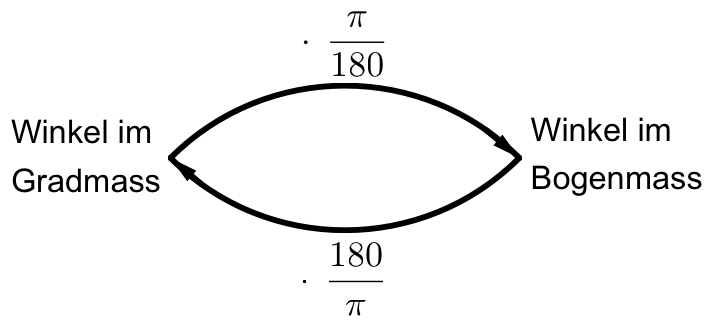
\includegraphics[scale=0.45]{UmrechnungGradRad.jpeg}
			\end{figure}
		\end{minipage}
	\end{satz}
	\begin{aufgabe}
		\begin{enumerate}[label=\alph*)]
			\item Berechne die folgenden Winkel im Bogenmass.
			\begin{table}[H]
				\centering
				\begin{tabular}{m{3cm}|m{0.8cm}|m{0.8cm}|m{0.8cm}|m{0.8cm}|m{0.8cm}|m{0.8cm}|m{0.8cm}|m{0.8cm}|m{0.8cm}}
					Winkel in Grad & $0^\circ$ & $30^\circ$ & $45^\circ$ & $60^\circ$ & $90^\circ$ & $120^\circ$ & $180^\circ$ & $270^\circ$ & $360^\circ$\\\hline
					Winkel in rad & & & & & & & & & \\
				\end{tabular}
			\end{table}
			\item Wandle in Bogenmass bzw. Gradmass um.
			\begin{enumerate}[label=\roman*)]\begin{multicols}{4}
					\item $135^\circ$
					\item $225^\circ$
					\item $35^\circ$
					\item $\frac{\pi}{5}$
					\item $\frac{3\pi}{5}$
					\item $\frac{7\pi}{9}$
					\item $\frac{\pi}{10}$
					\item $\frac{3\pi}{20}$
			\end{multicols}\end{enumerate}
		\end{enumerate}
	\end{aufgabe}\newpage



\subsection*{History}
\begin{table}[H]
	\centering
	\begin{tabular}{|p{13mm}|p{20mm}|p{30mm}|p{70mm}|}\hline
		%\multicolumn{4}{|l|}{History}\\\hline
		Version & Datum & Person & Bemerkung \\\hline
		$0.1$ & 22.12.2023 & Jonas Guler & Kapitel erstellt \\\hline
		$1.0$ & 28.04.2026 & Jonas Guler & kleine Korrekturen und Links als Hyperlinks ergänzt \\\hline
	\end{tabular}
\end{table}

\end{document}